\section{The Theory Underlying EASAL}
\label{sec:theory}

\begin{figure}[h]
\centering
\subfigure[Active constraint graph used to label a 2D node in (b); 
$(a_1, b_1)$ is the sole active constraint edge.]
{\label{fig:2DToy}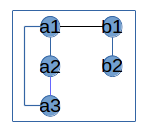
\includegraphics[width=0.2\linewidth]{\fig/1DACG.png}}
%\hskip0.1\linewidth
\subfigure[Stratification DAG of \exref{\toytwod}.]
{\label{fig:exampleStratification}
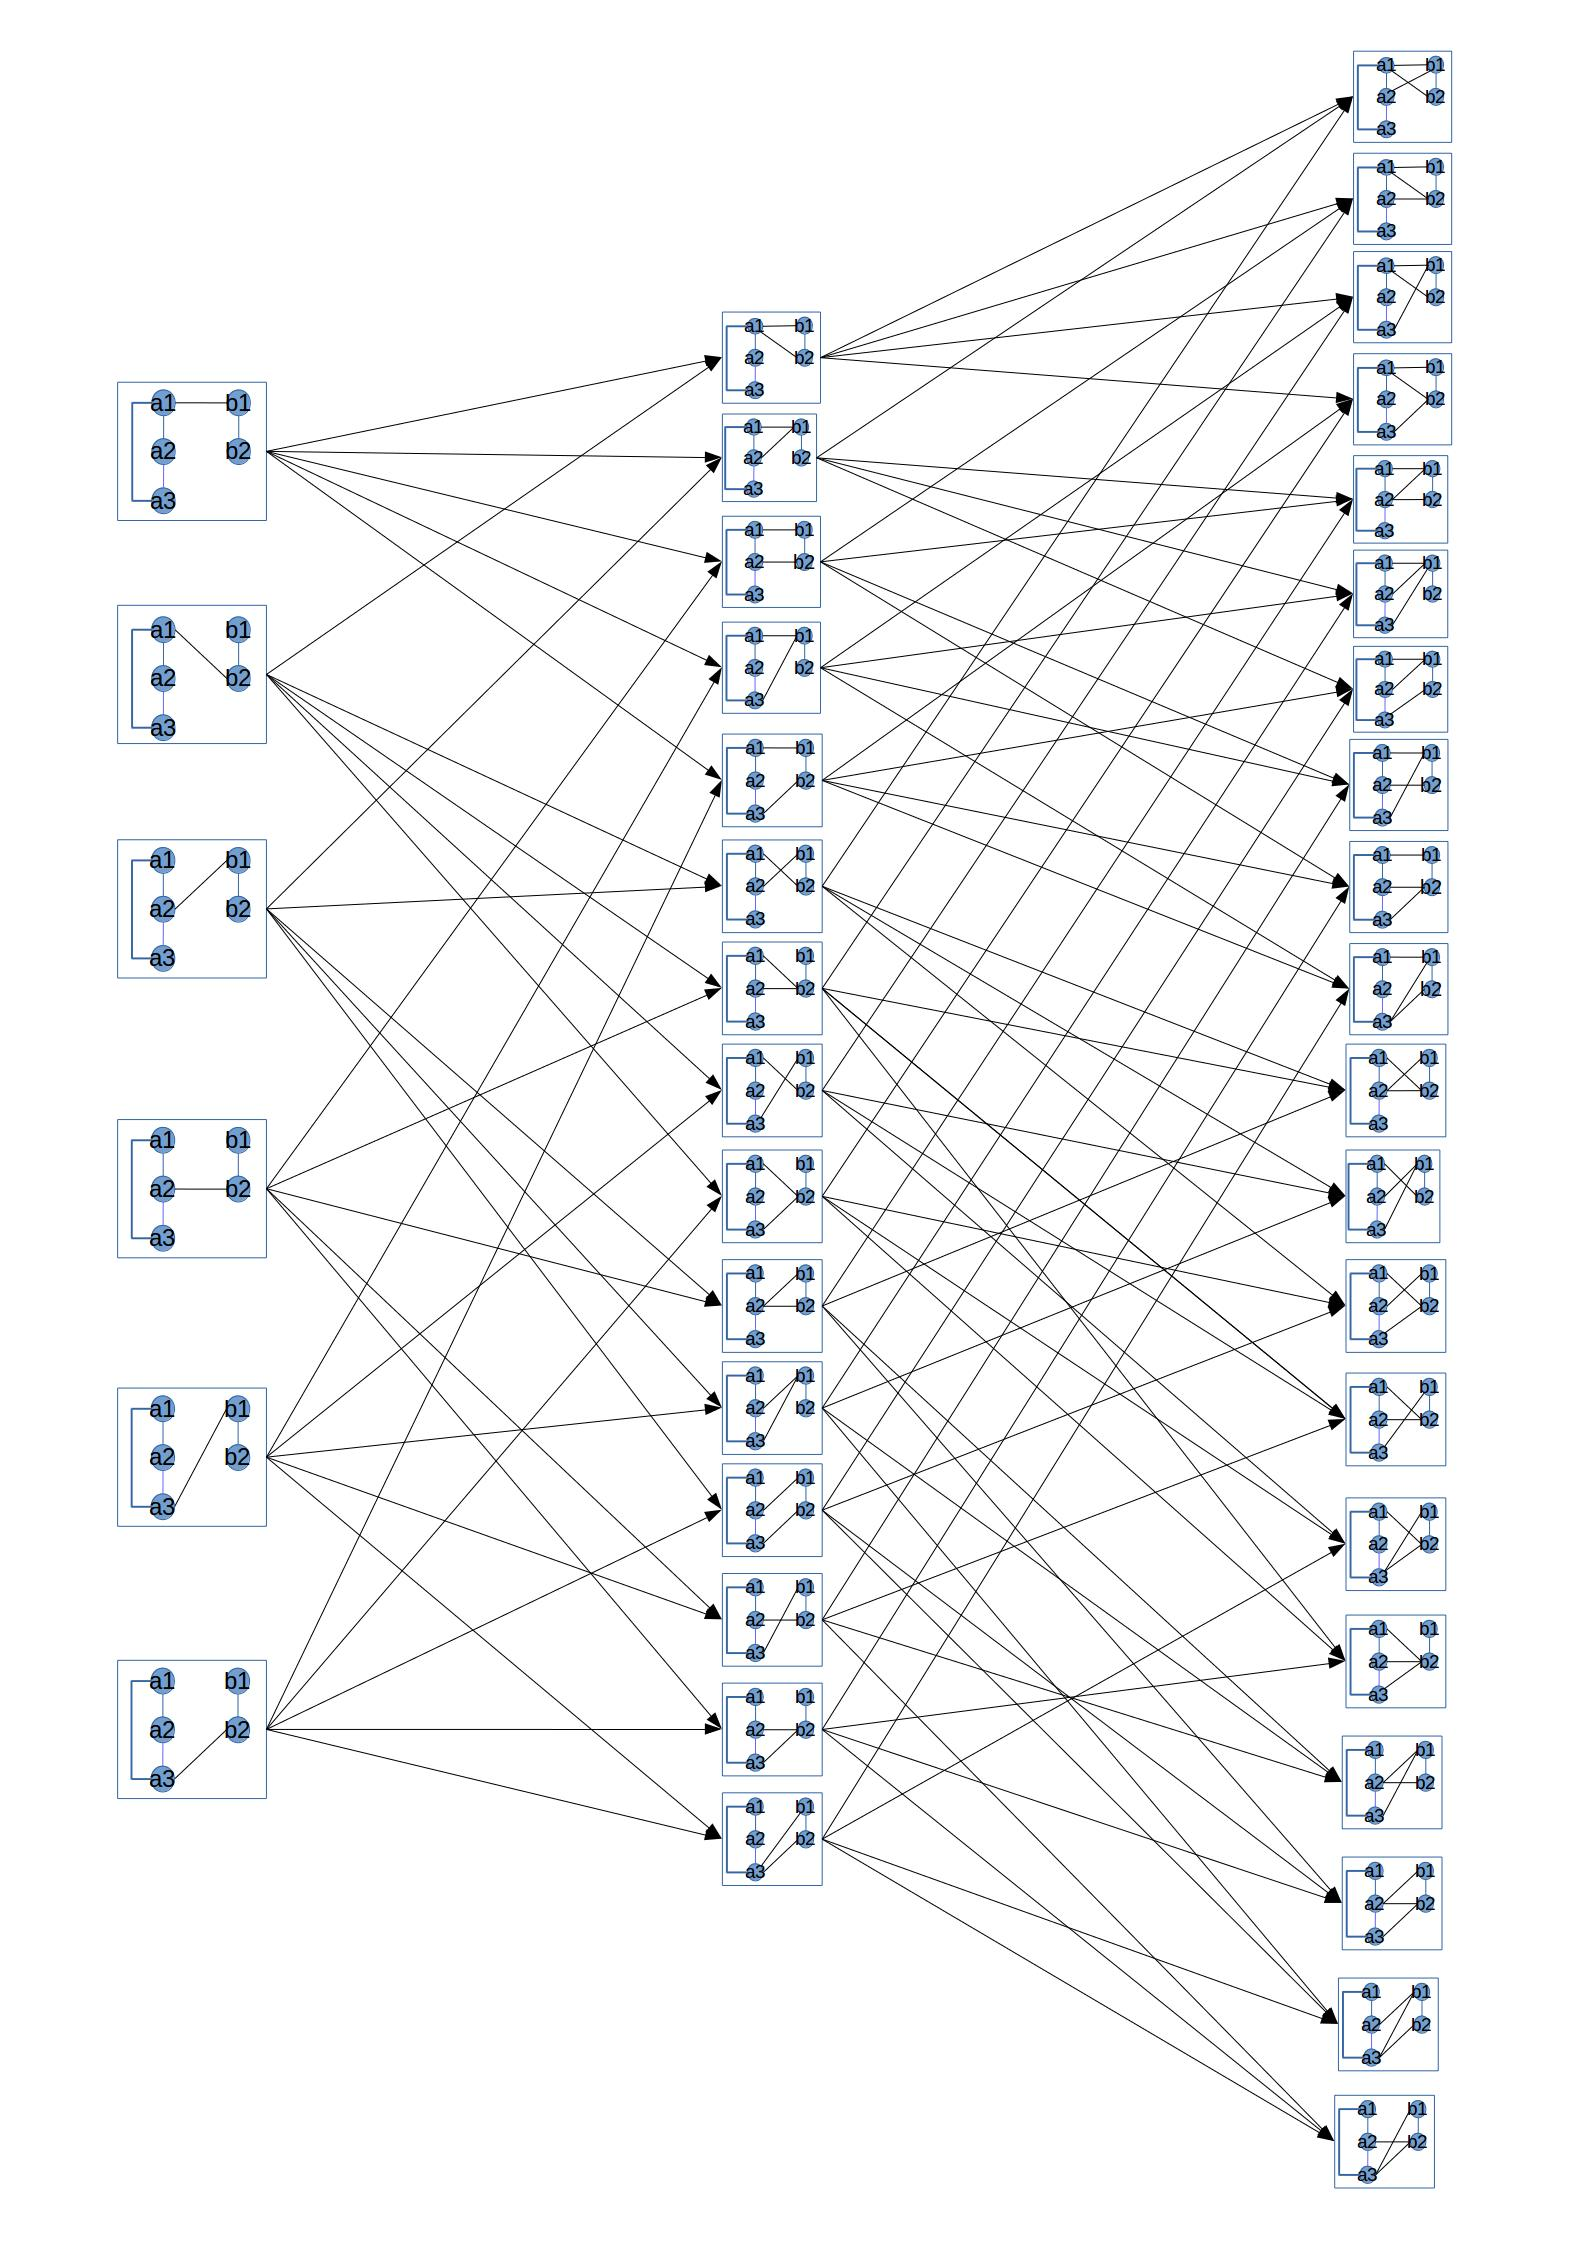
\includegraphics[width=0.7\linewidth]{\fig/2DConfigExample3-2.jpg}}
\caption{ Atlas (stratification) of the (toy-sized) configuration
space of \exref{\toytwod} of Section \ref{sec:toytwod}. (b) The nodes of the
DAG represent active constraint regions and DAG edges connect a region to a
boundary region, one dimension lower. Each node box displays the active
constraint graph of its corresponding region. The nodes in the leftmost column
represent 2D active constraint regions, i.e., they contain configurations with
two degrees of freedom. Adding an active constraint edge, yields 1D active
constraint regions (center column). Adding one more edge yields 0D regions,
each containing finitely many rigid configurations (rightmost column).}
\end{figure}

\begin{figure}[h]
\centering
%Fig1
\subfigure[Input to Problem (\cone, \ctwo).]{
\begin{overpic}[scale=.3,tics=10]{\fig/Input_white.png}
     \put (20,60) {\color{blue}{$A$}}
     \put (53,60) {\color{green}{$B$}}
\end{overpic}
\label{fig:pctreeInput}
}
%{\label{fig:pctreeInput}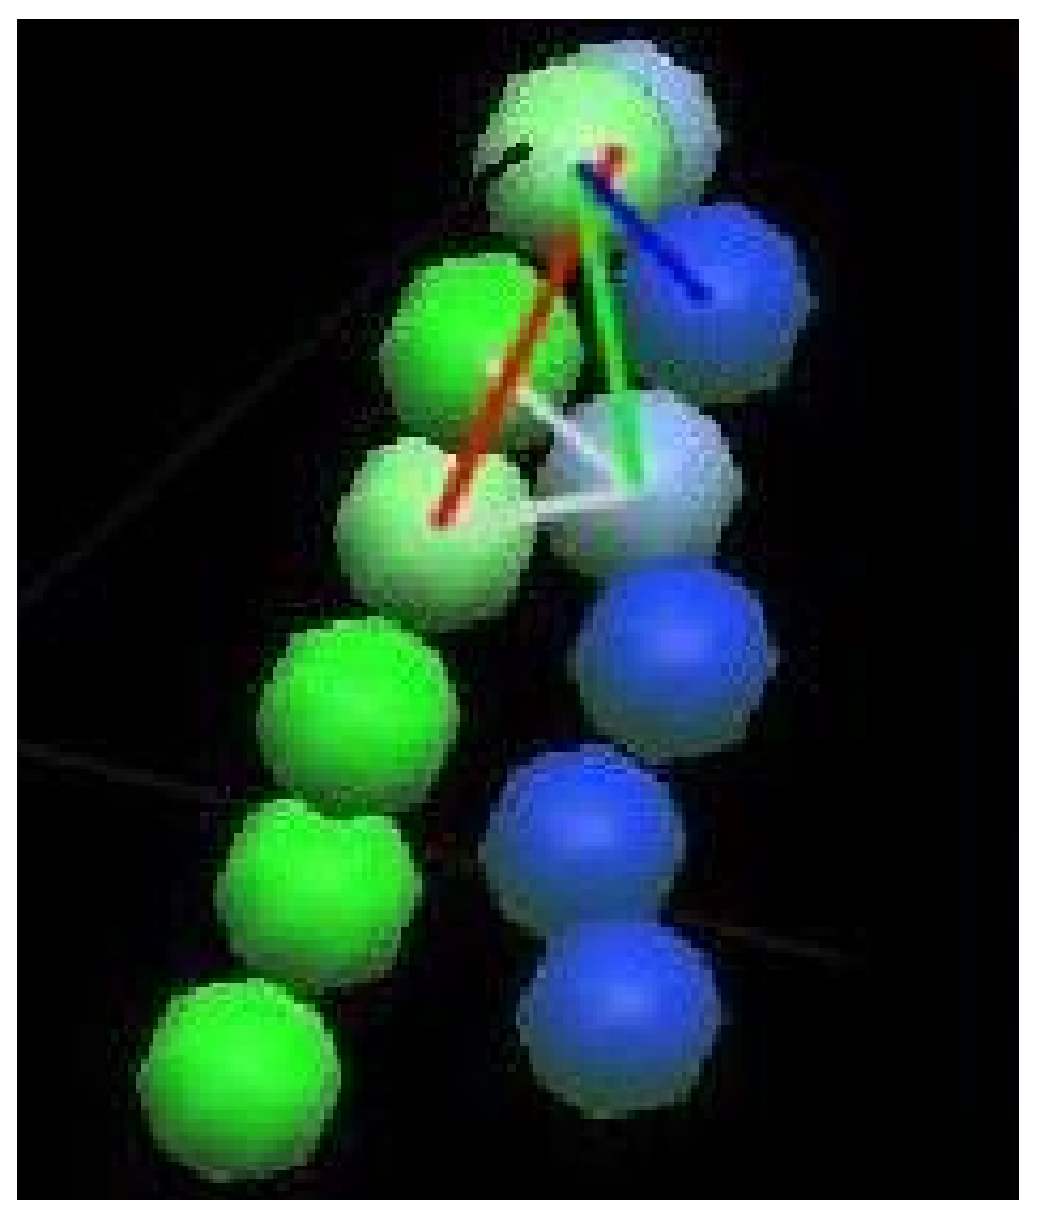
\includegraphics[width=0.2\linewidth]{\fig/Input.eps}}
%Fig2 
\subfigure[Active constraint regions in the atlas represented as nodes colored by their dimension, shown with their Cayley configuration spaces (see full caption below).]{
\begin{overpic}[scale=.3,tics=10]{\fig/CayleySpaces_white.png}
     %\put (80,80) {\color{white}{1d cayley}}
     \put (50,75) {\color{grayoned}{1D Cayley}}
     \put (75,35) {\color{grayoned}{1D Cayley}}
     \put (75,28) {\color{grayoned}{1D node}}
     \put (76,20) {\color{green2d}{2D Cayley}}
     \put (76,15) {\color{green2d}{with hole}}
     \put (55,38) {\color{green2d}{2D node}}
     \put (08,80) {\color{yelloworange}{3D Cayley}}
     \put (48,05) {\color{yelloworange}{3D Cayley}}
     \put (42,15) {\color{yelloworange}{3D node}}
     \put (5,10) {\color{red}{4D node}}
\end{overpic}
\label{fig:pctreeSpace}
}
%{\label{fig:pctreeSpace}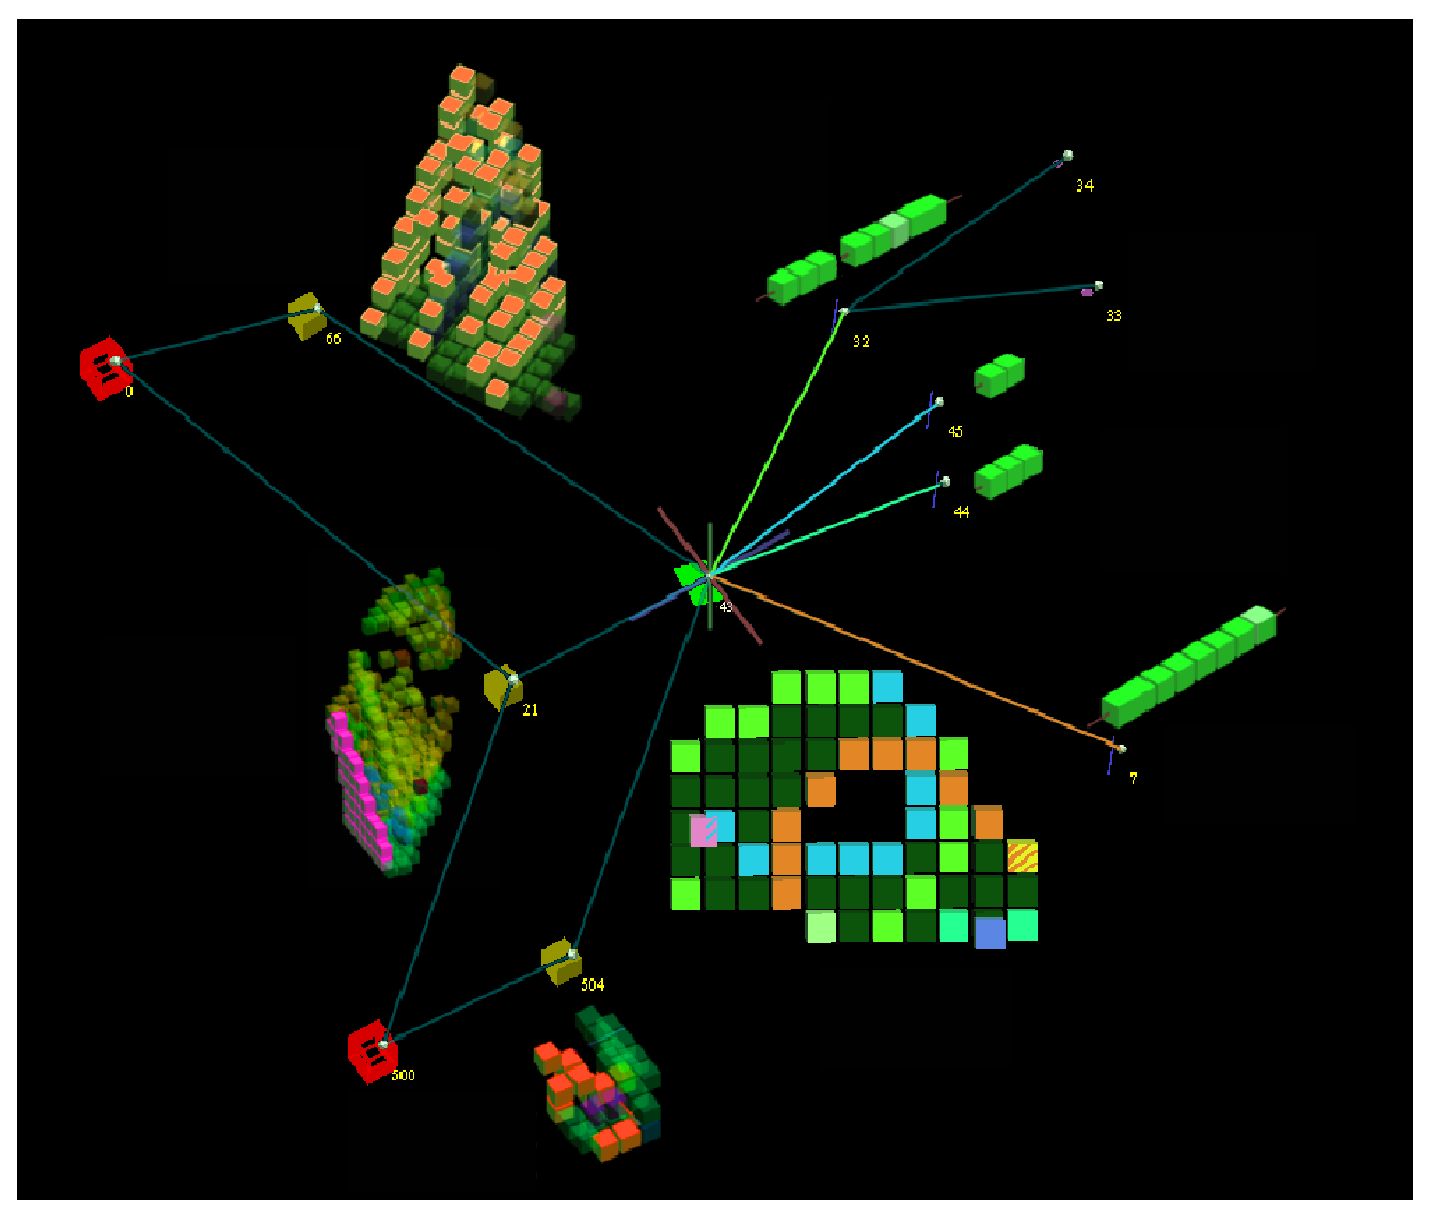
\includegraphics[width=0.4\linewidth, height=0.3\linewidth]{\fig/CayleySpaces.eps}}
\subfigure[Active constraint regions in the atlas represented as nodes colored by their dimension, shown with their active constraint graphs.]{
\begin{overpic}[scale=.3,tics=10]{\fig/ACG_white.png}
     \put (69,18) {\color{grayoned}{5 active}}
     \put (65,14) {\color{grayoned}{constraints}}
     %\put (50,75) {\color{white}{5 contacts}}
     %\put (70,45) {\color{white}{1d node}}
     \put (75,28) {\color{grayoned}{1D node}}
     \put (48,27) {\color{green2d}{4 active}}
     \put (46,23) {\color{green2d}{constraints}}
     \put (40,37) {\color{green2d}{2D node}}
     %\put (10,80) {\color{yellow}{3 contacts}}
     \put (20,2) {\color{yelloworange}{3 active constraints}}
     \put (42,15) {\color{yelloworange}{3D node}}
     \put (5,10) {\color{red}{4D node}}
\end{overpic}
\label{fig:pctreeACG}
}
%{\label{fig:pctreeACG}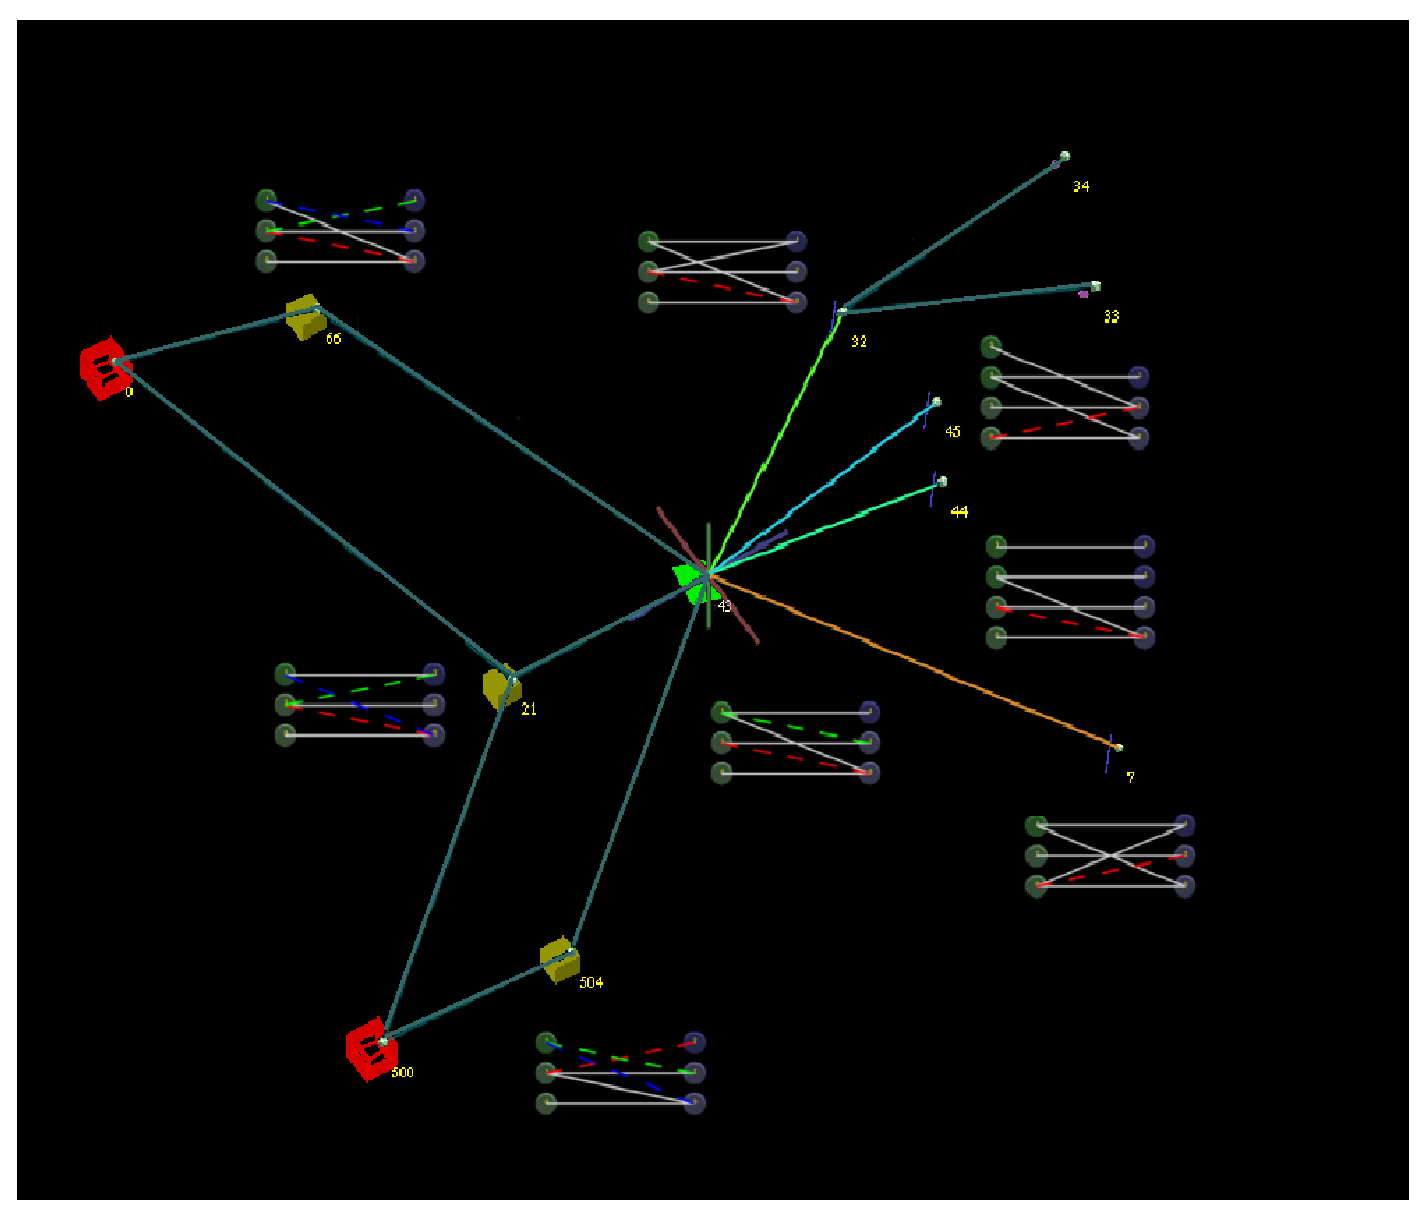
\includegraphics[width=0.4\linewidth,height=0.3\linewidth]{\fig/ACG.eps}}
%Fig3
%Fig4
\subfigure[Active constraint regions in the atlas represented as nodes colored by their dimension, shown with Cartesian configuration sweep views(see full caption below).]{
\begin{overpic}[scale=.25,tics=10]{\fig/Sweeps_white.png}
     %\put (78,18) {\color{white}{5 contacts}}
     %\put (50,75) {\color{white}{5 contacts}}
     %\put (70,45) {\color{white}{1d node}}
     \put (15,85) {\color{yelloworange}{sweep views of different flips}}
     \put (75,25) {\color{grayoned}{1D node}}
     %\put (47,27) {\color{green}{4 contacts}}
     \put (40,40) {\color{green2d}{2D node}}
     %\put (10,80) {\color{yellow}{3 contacts}}
     %\put (40,2) {\color{yellow}{3 contacts}}
     %\put (20,15) {\color{yelloworange}{3D node}}
     \put (18,17) {\color{yelloworange}{3D node}}
     \put (0,10) {\color{red}{4D node}}
\end{overpic}
\label{fig:pctreeSweep}
}
%{\label{fig:pctreeSweep}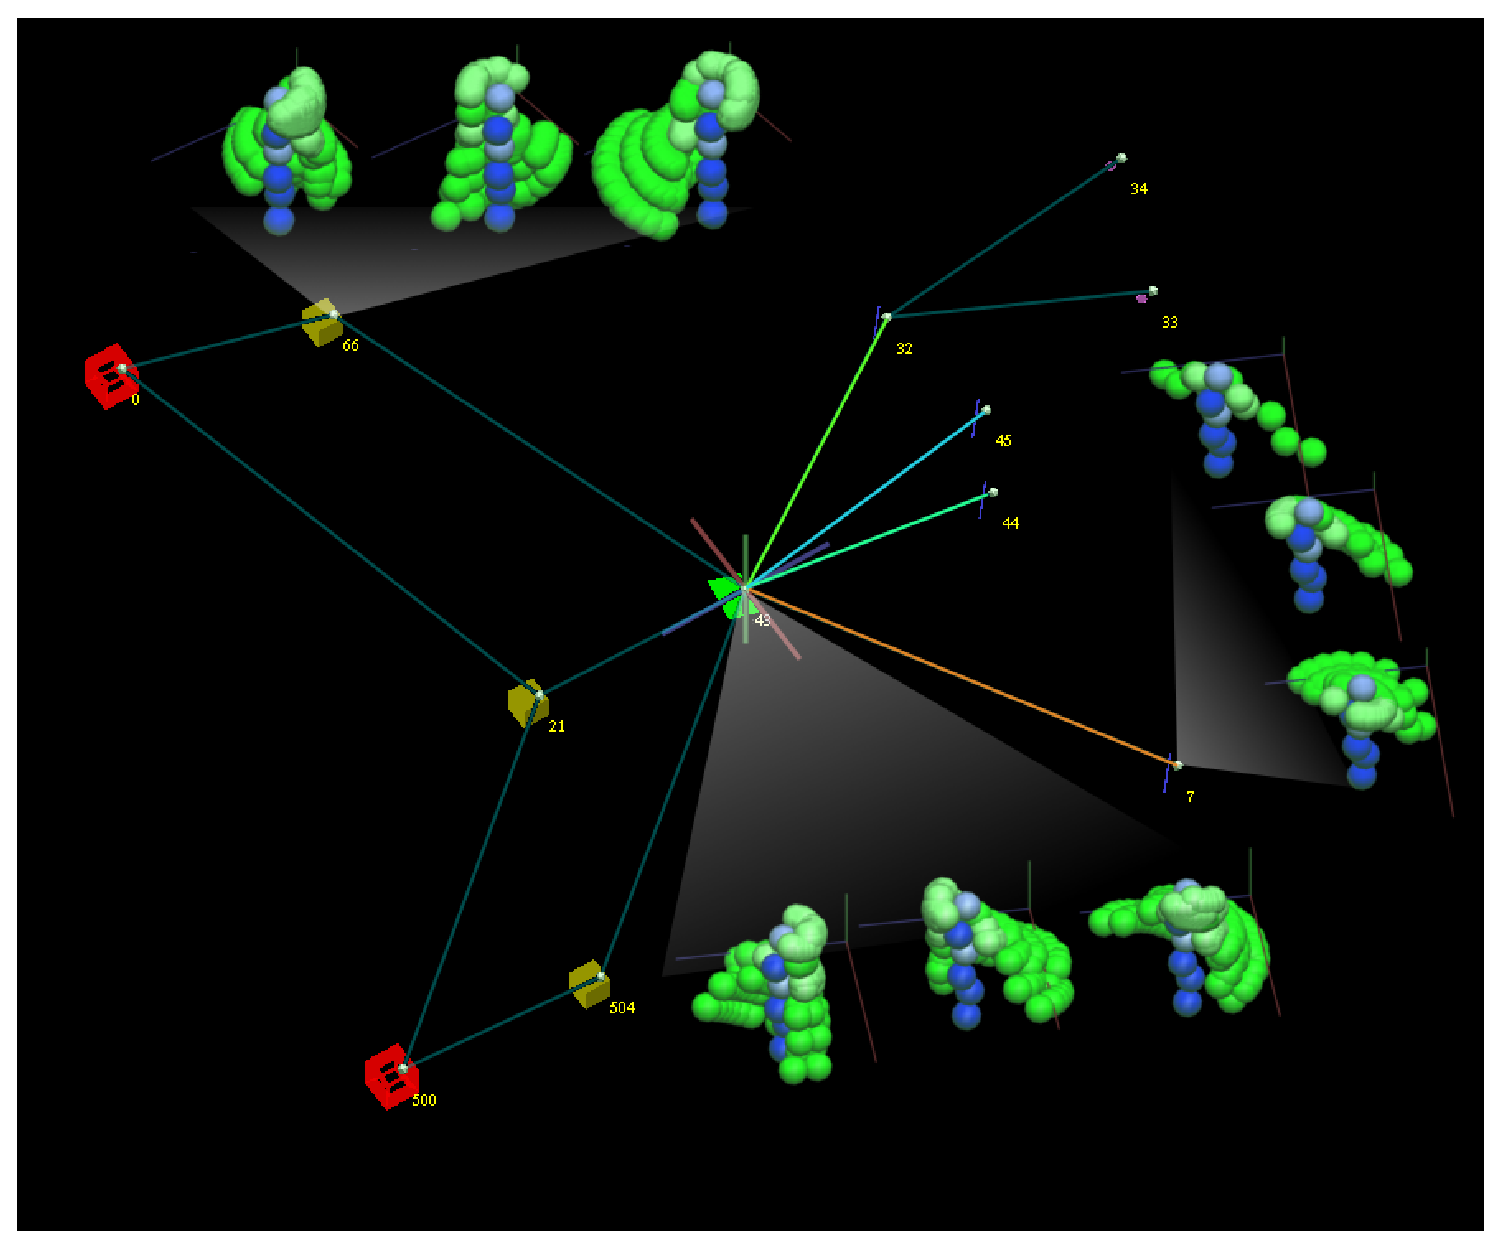
\includegraphics[width=0.4\linewidth, height=0.3\linewidth]{\fig/Sweeps.eps}}
\caption{\footnotesize 
(b), (c), and (d) show different views of a portion of the atlas centered on a
2D active constraint region.  (b) The grid of little cubes next to each node
delineates the Cayley configuration space of that region. Each little cube is a
Cayley point or a Cayley configuration.  Consider the 2D active constraint
region in the center.  This region has has no Cayley points in the middle (a
hole) since every realization of these Cayley points violates \cone. These
violations are caused by point pairs that are neither Cayley parameters nor
edges of the active constraint graph. Such hole regions typically also have a
convex Cayley parametrization.  The Cayley points highlighted with a different
color are points adjacent to their child (boundary) regions albeit using
different Cayley parameters.  (d) Each sweep view is the union of realizations,
one per Cartesian configuration in the corresponding node. Each sweep view
shows a different flip (defined in Section \ref{sec:realization}) of the Cayley
configuration space of the corresponding node. 
}
\label{fig:NestedRegions}
\end{figure}
%\old{ OLD caption of Fig 2 -- moves figure to end if I leave it in!!
%{\bf Parent and child (boundary) regions a 2D region}
%of the atlas \textbf{for} the input shown in (a).  Figures (b), (c), and (d) depict the
%node of the 2D region (green) in the center. The 2D active constraint region is
%a boundary region of the 3D active constraint regions shown in light green. The
%boundaries of the 2D active constraint region are the 1D active constraint
%regions shown in blue.\\
%(a) The input to the constraint system. 
%(b) The grid of cubes next to each node delineates the Cayley configuration
%space of the region. The 2D region has a hole cut out. The infeasible region in
%the interior of the hole is caused by violation of \cone involving a point pair
%that is not a Cayley parameter. The violation occurs in every realization of
%the Cayley points within. This hole region typically also has a convex Cayley
%parametrization; the boundary of each such hole corresponds to a newly active
%constraint (child region). In fact, such boundary regions are encountered even
%when a single realization of a Cayley point violates \cone.
%(c) Nodes labeled by their active constraint graphs. 
%(d) The sweep view shows the set $A$ (a many-atom molecule) shown in blue and
%all feasible realizations $T(B)$ traced out of the second set $B$ in green.
%} 

The EASAL software is based on the theoretical concepts described in this section. 
We explain and illustrate EASAL's three strategies below. The reader will find
the video at \url{http://www.cise.ufl.edu/∼ rprabhu/EASALvideo.mpg} useful to understand the following. 


%\begin{figure}[h]
%\centering
%Fig1
%\subfigure[Input to Problem (\cone, \ctwo).]
%{\label{fig:pctreeInput}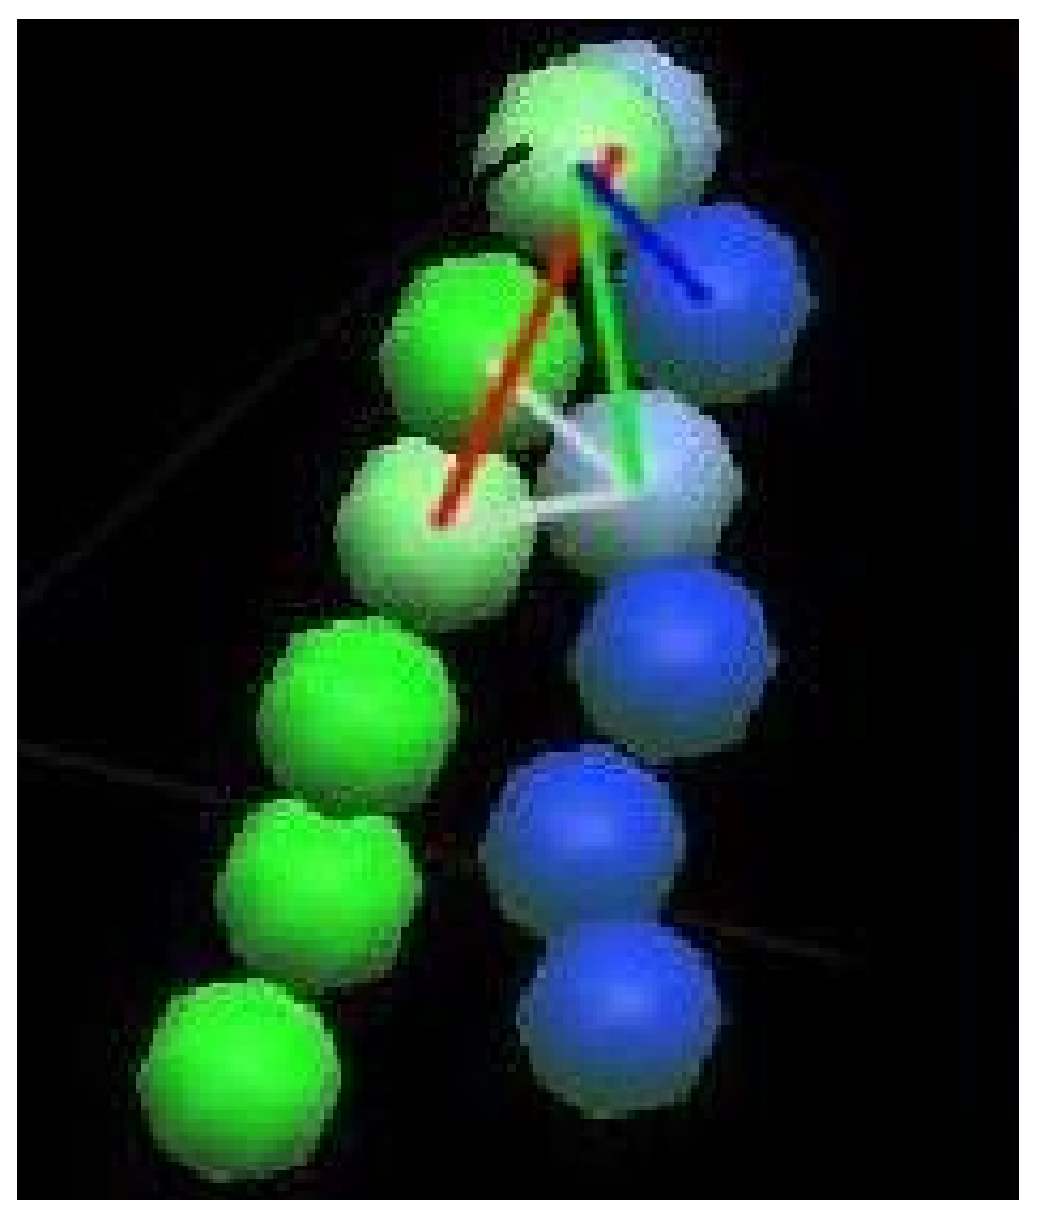
\includegraphics[width=0.2\linewidth]{\fig/Input.eps}}
%Fig2 
%\subfigure[Atlas node regions with their Cayley configuration spaces.]
%{\label{fig:pctreeSpace}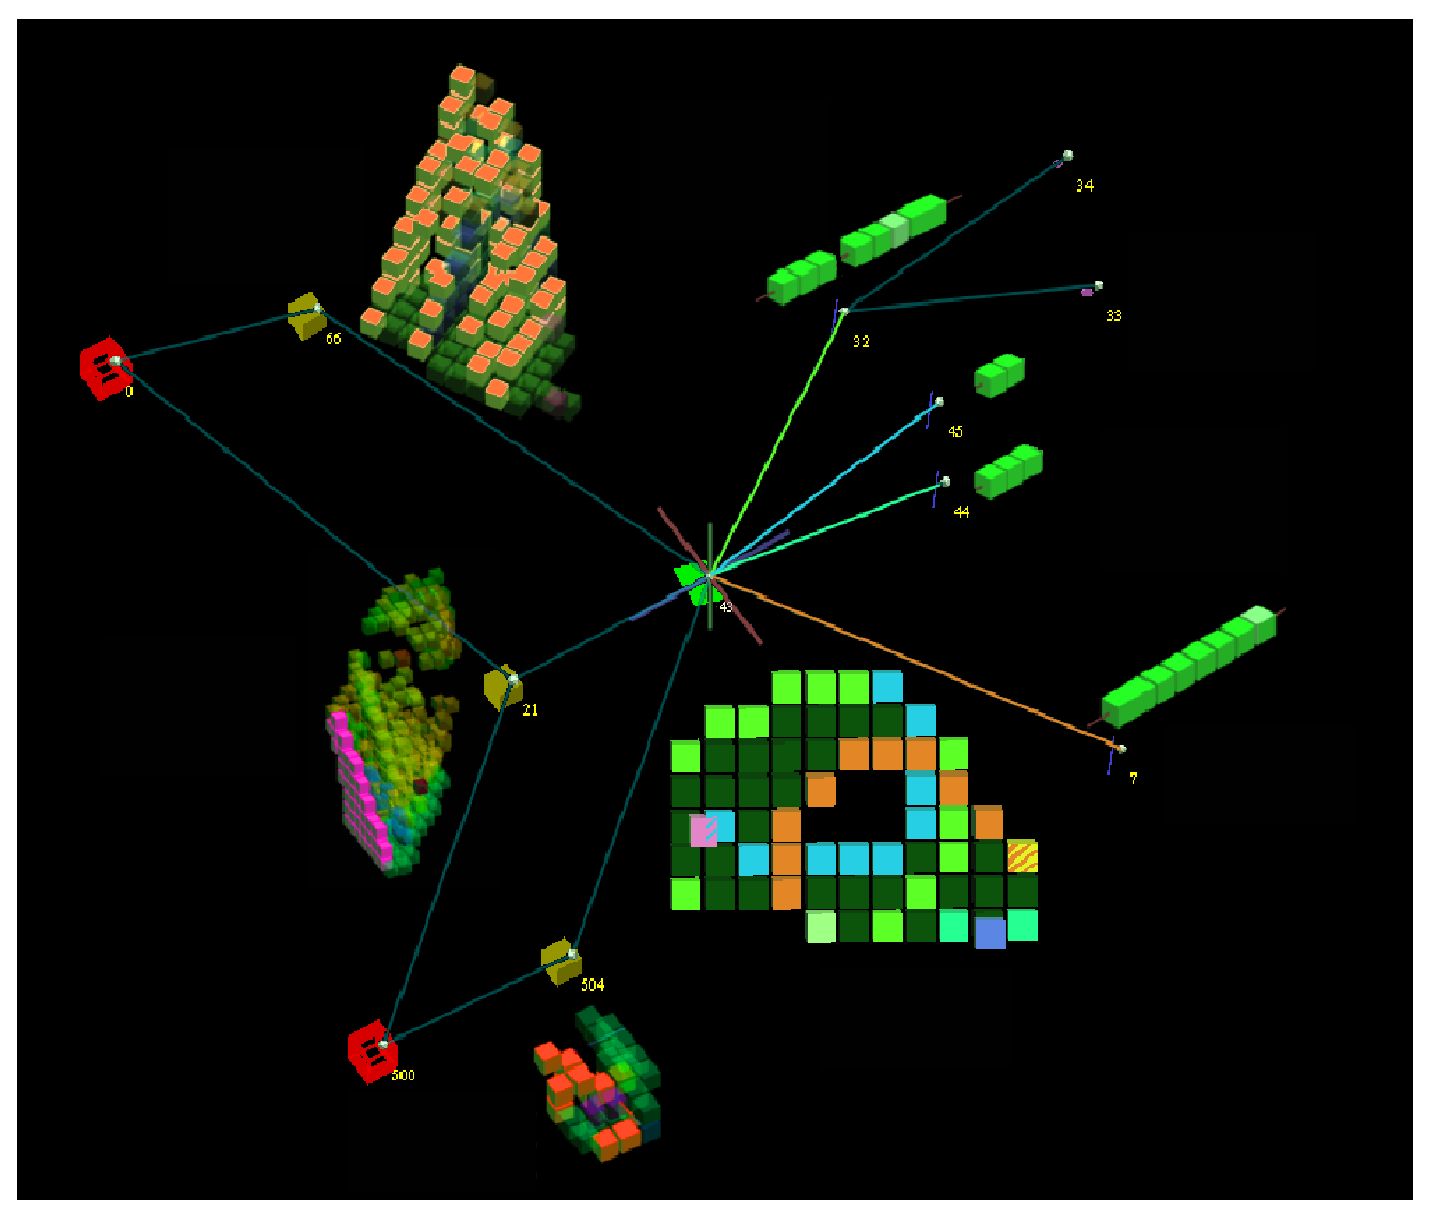
\includegraphics[width=0.4\linewidth, height=0.3\linewidth]{\fig/CayleySpaces.eps}}
%\subfigure[Atlas nodes with their active constraint graphs.]
%{\label{fig:pctreeACG}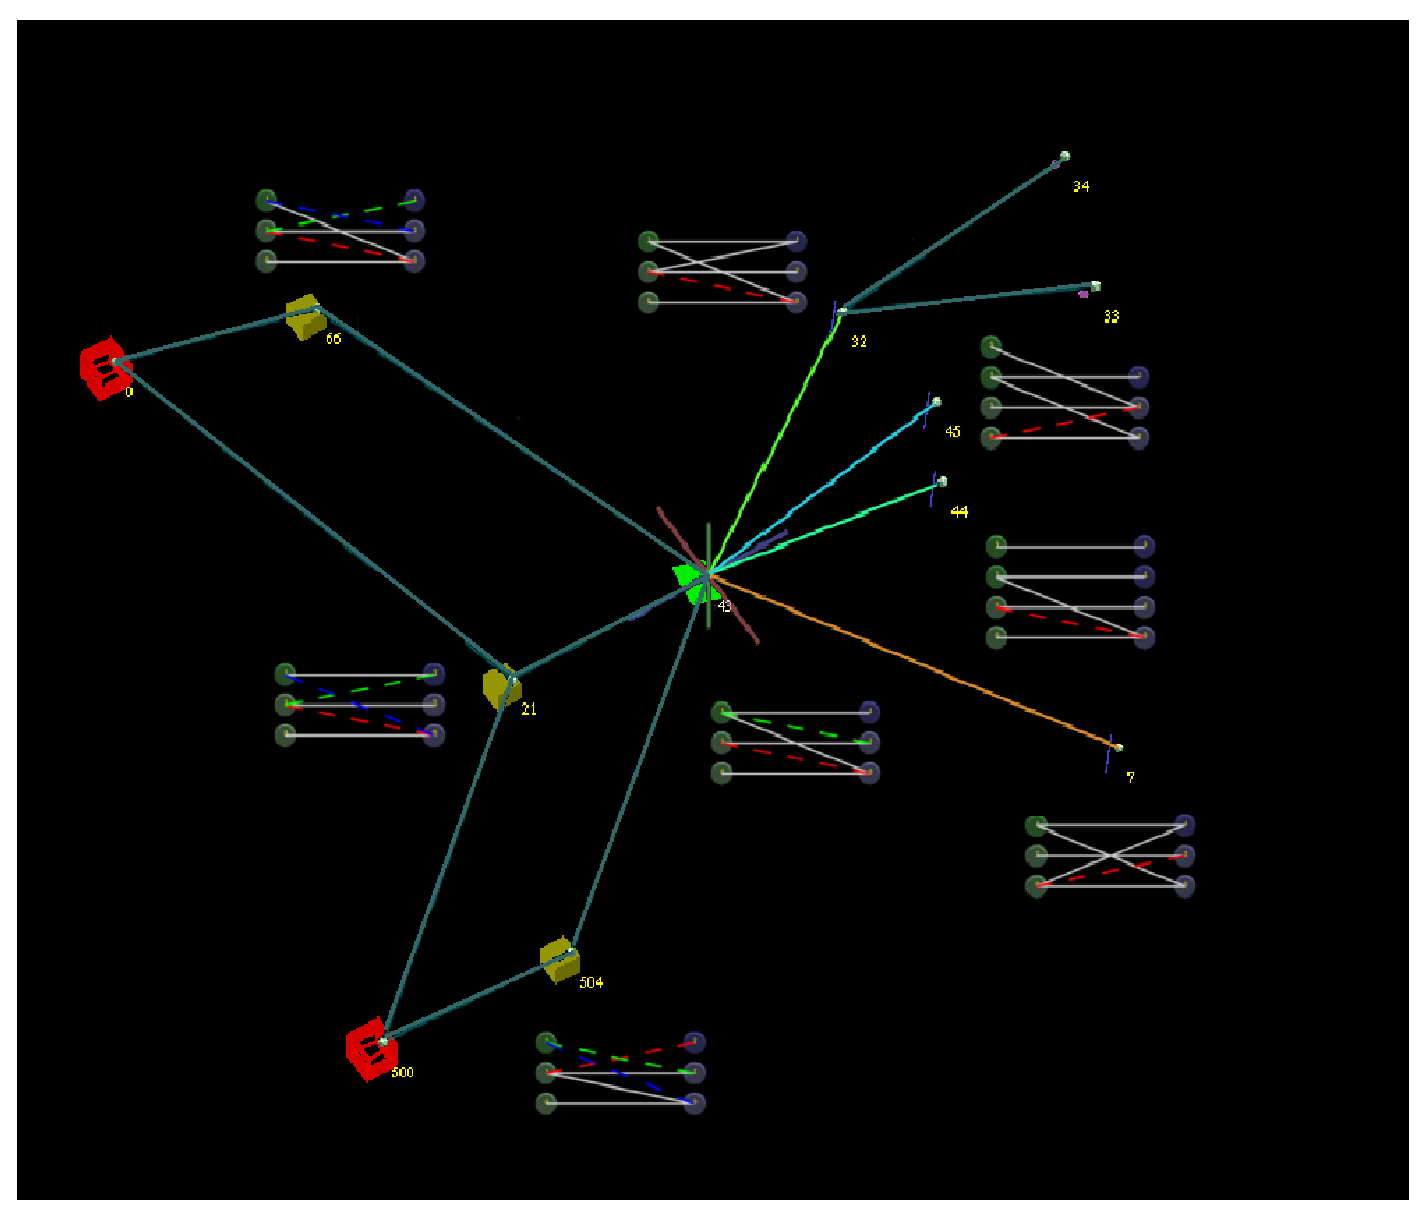
\includegraphics[width=0.4\linewidth,height=0.3\linewidth]{\fig/ACG.eps}}
%Fig3
%Fig4
%\subfigure[Atlas node regions with Cartesian configuration sweep views.]
%{\label{fig:pctreeSweep}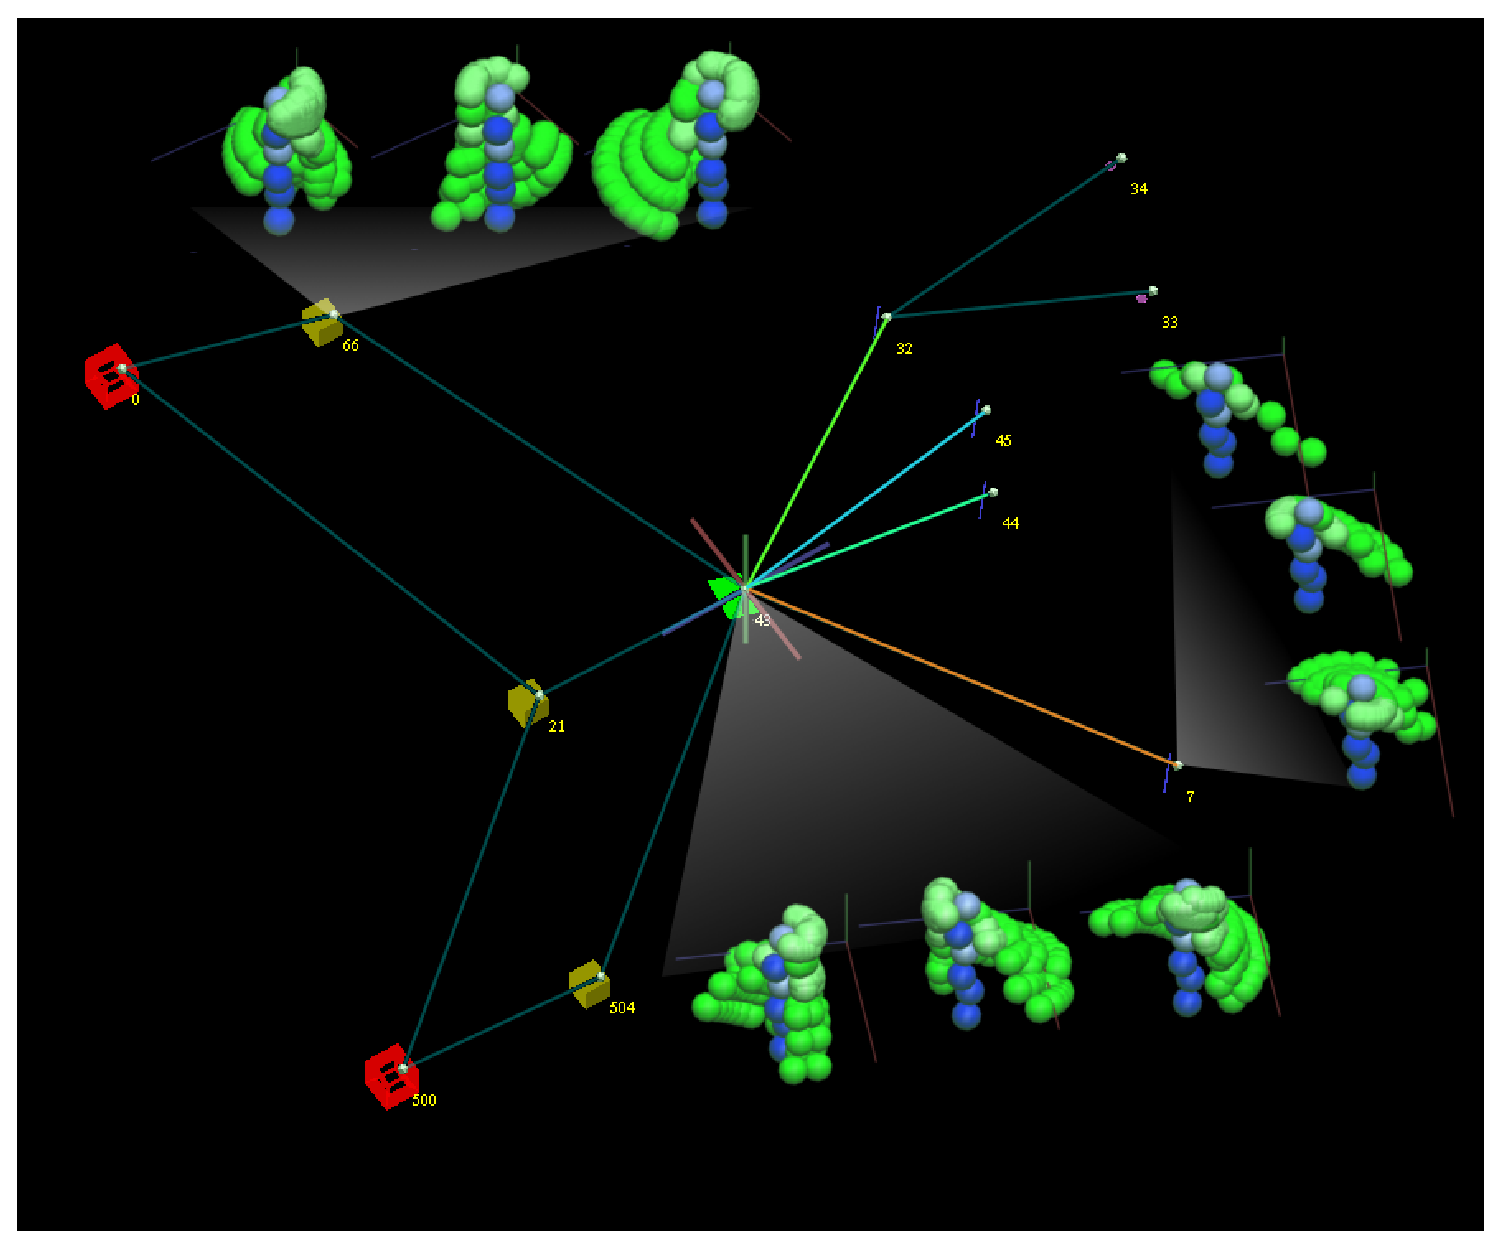
\includegraphics[width=0.4\linewidth, height=0.3\linewidth]{\fig/Sweeps.eps}}
%\caption{\footnotesize {\bf Parent and child (boundary) regions of a 2D region}
%of the atlas of the input shown in (a).  Figures (b), (c), and (d) depict the
%node of the 2D region (green) in the center. The 2D active constraint region is
%a boundary region of the 3D active constraint regions shown in light green. The
%boundaries of the 2D active constraint region are the 1D active constraint
%regions shown in blue.\\
%(a) The input to the constraint system. 
%(b) Nodes labeled by their active constraint graphs. 
%(c) The grid of cubes next to each node delineates the Cayley configuration
%space of the region. The 2D region has a hole cut out. The infeasible region in
%the interior of the hole is caused by violation of \cone involving a point pair
%that is not a Cayley parameter. The violation occurs in every realization of
%the Cayley points within. This hole region typically also has a convex Cayley
%parametrization; the boundary of each such hole corresponds to a newly active
%constraint (child region). In fact, such boundary regions are encountered even
%when a single realization of a Cayley point violates \cone.
%(d) The sweep view shows the set $A$ (a many-atom molecule) shown in blue and
%all feasible realizations $T(B)$ traced out of the second set $B$ in green.} 
%\label{fig:NestedRegions}
%\end{figure}


%\footnote{Source code, optional GUI and user/developer guide available at
%\url{https://bitbucket.org/geoplexity/easal} \cite{easalSoftware}\\A video
%demonstrating the working of EASAL, is available at
%\url{http://www.cise.ufl.edu/~rprabhu/EASALvideo.mpg} \cite{easalVideo}} 

\subsection{Strategy 1: Atlasing and Stratification}
\label{sec:stratification}

EASAL's first strategy is to partition and stratify the Cartesian configuration
space into regions $R$ called the active constraint regions, each labeled by
its \emph{active constraint graph} (See \figref{fig:2DToy}).  Consider the set
of points participating in the active constraints that define $R$. Let $V_R$ be
any minimal superset of points that supports additional constraints, of type
\ctwo, to locally fix (generically rigidify) the two point-sets with respect to
each other.  Now, $V_R$ is taken to be the set of vertices of the active
constraint graph of $R$. An edge of the active constraint graph represents
either (i) one of the active constraints that define $R$ or (ii) a vertex pair
in $V_R$ that lies in the same point-set $A$ (or $B$) in Problem (\cone, \ctwo). Notice that building the active
constraint graph of $R$ reduces to picking a minimal graph isomorph from
\figref{fig:3-trees} containing the active constraints that define $R$.

The active constraint regions are organized as a partial order (directed
acyclic graph or DAG, see \figref{fig:exampleStratification} and
\figref{fig:pctreeACG}), that captures their dimensions and boundary
relationships. In particular, the active constraint graph of a region is a
subgraph of the active constraint graph of its boundary regions; and the
co-dimension of a region is generically the number of active constraint edges.
The analysis of the graph benefits from the following concepts of combinatorial
rigidity (we additionally refer the reader to \cite{CombinatorialRigidity}).

A \emph{linkage} is a graph, $G = (V, E)$, of vertices and edges, with an
assignment of lengths, $\gamma: E \rightarrow \mathbb{R}$, for each edge. A
(Euclidean) \emph{realization} of a linkage in $\mathbb{R}^3$ is an assignment
of points in $\mathbb{R}^3$ to vertices (factoring out the three rotations and
three translations of SE(3)) such that the Euclidean distance between pairs of
points are the given edge lengths $\gamma$. A realization is said to be
\emph{rigid} if there is no other realization in its neighborhood that has the
same edge lengths. A graph is said to be rigid if a generic linkage realization
of the graph is rigid. Otherwise, the graph is said to be flexible (not rigid).
A rigid linkage generically has finitely many realizations. A graph is said to
be \emph{minimally rigid}, \emph{well constrained} or \emph{isostatic} if it is
rigid and the removal of any edge causes it to be flexible. When the
realization is rigid, all non-edges have locally fixed lengths and are said to
be locally \emph{implied} or \emph{dependent}.  If the graph $G$ arises as an
active constraint graph for Problem (\cone, \ctwo) with the active constraint
edges being assigned length intervals, we obtain an \emph{active constraint
linkage}. In this paper we treat active constraint linkages just like linkages
while analyzing generic rigidity properties. 




\begin{figure}[h]
\centering
      \subfigure[20 atom input]{
         \label{fig:3Input}
         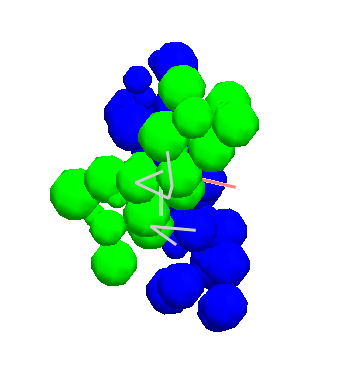
\includegraphics[scale=0.2]{\fig/Figure3Input.png}
         }
      %\fbox{\subfigure{\label{fig:3Input}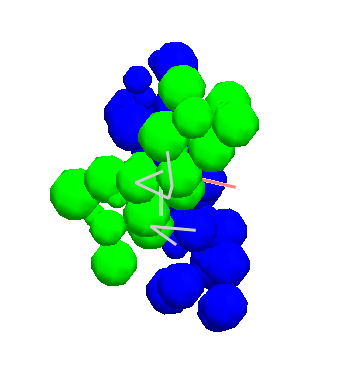
\includegraphics[scale=0.2]{\fig/Figure3Input.png}}}
	%\renewcommand{\thesubfigure}{(a)}
	\subfigure[Realization sweep view]{
	\label{fig:RealizationSweepView}
	\begin{overpic}[scale=.2,tics=10]{\fig/sweepview.eps}
		\linethickness{3pt}
		\put(56,76){\color{black}\vector(1,1){18}}
		\put(36,73){\color{black}\vector(1,3){8}}
		\put (20,100) {\color{black}{$T(B)$ sweep}}
		\put (76,95) {\color{black}{$A$ fixed}}
	\end{overpic}
        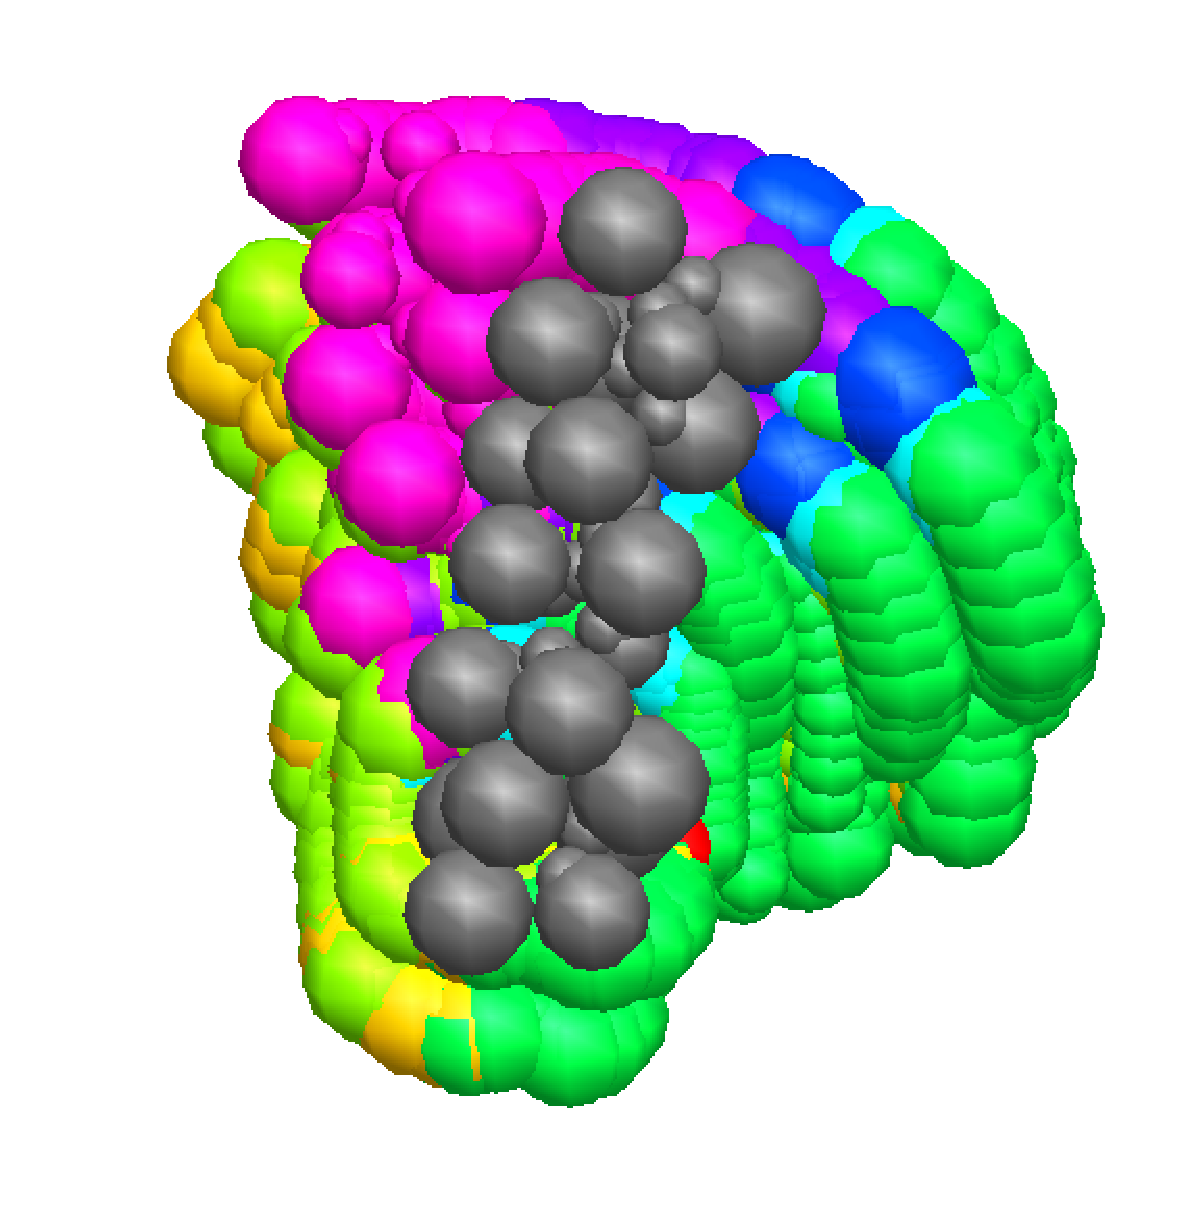
\includegraphics[scale=0.2]{\fig/sweepboundaries.eps}
        }
	\phantom{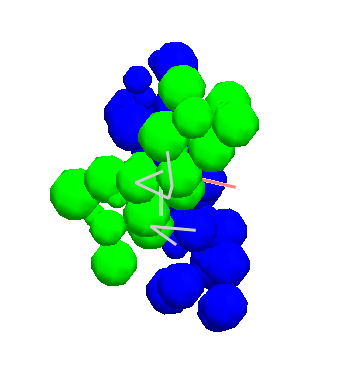
\includegraphics[scale=0.2]{\fig/Figure3Input.png}}
	%\renewcommand{\thesubfigure}{(c)}
	\subfigure[Cayley configuration space view]{
           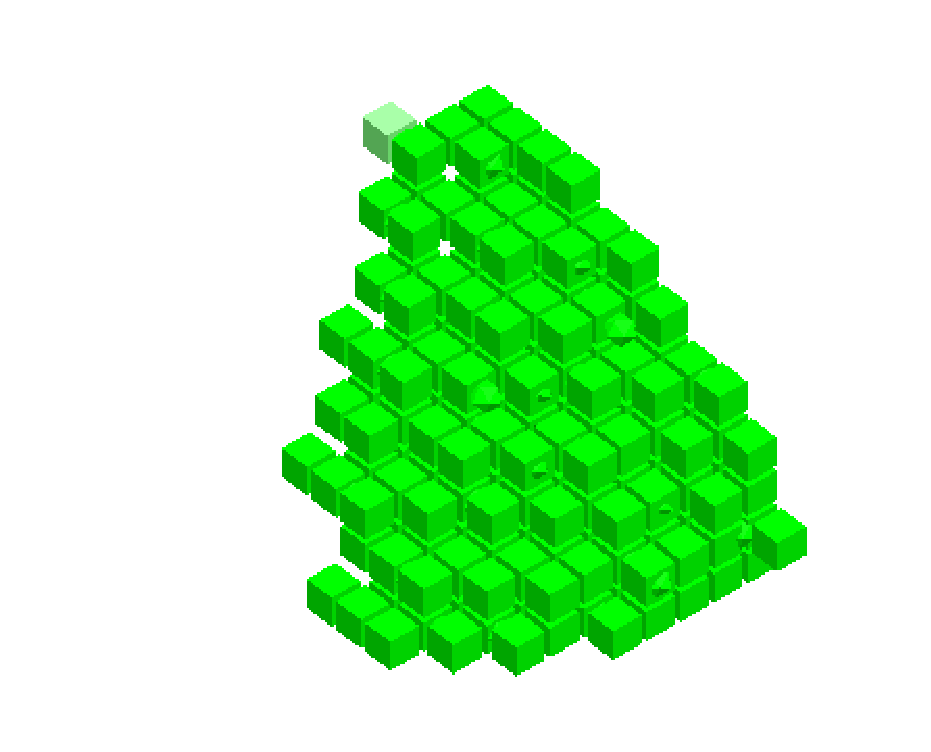
\includegraphics[scale=0.35]{\fig/space.eps}
           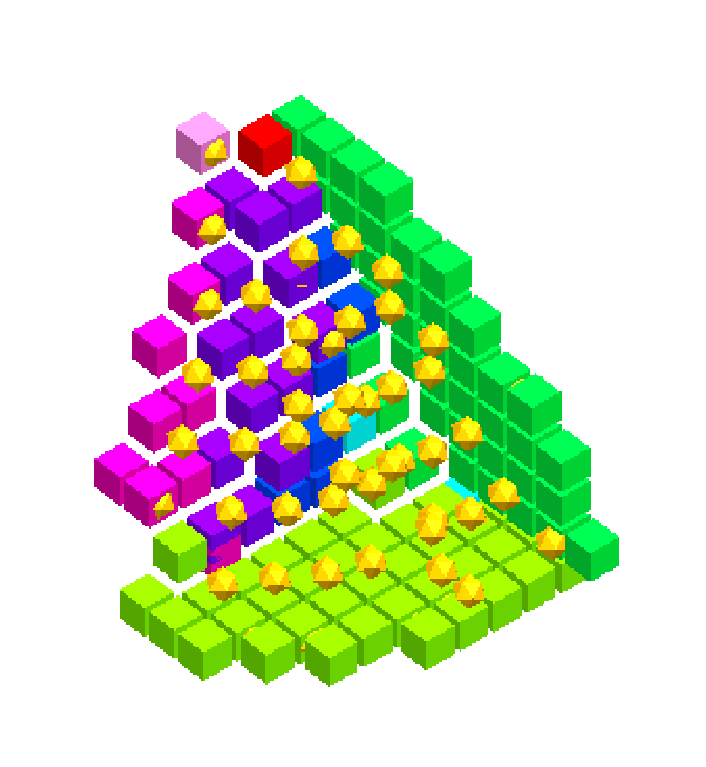
\includegraphics[scale=0.35]{\fig/spaceboundaries.eps}
           }
\caption{ Realization sweep view and Cayley configuration view of \exref{\bighelix}.
(b) Sweep of realizations $T(B)$ for fixed $A$ in a 3D active constraint
region. (b,\IR) Same view with $T(B)$ color coded to show
realizations adjacent to lower dimensional boundary regions where a new
constraint becomes active.
%, or yellow for the interior.} 
(c) Each cube represents one Cayley configuration with
at least one realization. % (shown in the sweep \IT,\IL).  
(c,\IR) Only those Cayley points adjacent to child boundary regions are color coded as in (b, \IR),
except for the yellow ones, shown as icosahedra, which are placed there as
witness points (see Sections \ref{sec:exploration}, \ref{sec:aposteriori} and \ref{sec:raytracing}) 
by parent regions, since this region is a boundary of those parent regions.
}
\label{fig:boundarySweeps}
\end{figure}

The degrees of freedom (dof) of a graph (linkage) is the minimum number of
edges whose addition makes it rigid. Thus, the number of degrees of freedom is
the same as the generic (effective) dimension of the realization space of a
(active constraint) linkage of the graph. In $\mathbb{R}^3$, Maxwell's theorem
\cite{maxwell} states that rigidity of a graph $G=(V,E)$, implies that $|E| \ge
3|V| - 6$ (in $\mathbb{R}^2$, $|E| \ge 2|V| - 3$). If the edges are
independent, this ensures minimal rigidity.

When $k=2$, the effective dimension of an active constraint region plus the
number of active constraints is always 6, i.e., the number of active
constraints generically determines the co-dimension of the region. This is
because, in Problem (\cone, \ctwo), generically, implied non-edges are not active constraints, i.e., the
active constraint edges are not implied by (dependent on) the rest of the
active constraint graph. Inactive constraints (implied or not) do not restrict
the dimension of active constraint regions. For the special case of Problem
(\cone, \ctwo), in which sets $A$ and $B$ are centers of non intersecting 
spheres, these genericity assumptions are an unproven conjecture, for which
counterexamples haven't been encountered.

Employing these concepts, EASAL is able to use a classical notion called the
Thom-Whitney stratification \cite{Kuo} of (effective) dimensional regions of a
semi-algebraic set to stratify the configuration space atlas. In the atlas, DAG
edges between two nodes indicate a boundary relationship: a lower dimensional
child region is the boundary of a parent region one dimension higher (one fewer
active constraint). Thus, the atlas is organized into strata, one for each
(effective) dimension, and DAG edges exist only between adjacent strata. In
Section \ref{sec:exploration}, we describe in detail the algorithm used for
atlasing and stratification of the configuration space.

\subsubsection{\toytwod}
\label{sec:toytwod}
Consider Problem (\cone, \ctwo) in $\mathbb{R}^2$ with two point-sets $A$ and
$B$; $A$ contains three points - $a_1$, $a_2$, and $a_3$ and $B$ contains two
points - $b_1$ and $b_2$. The ambient space is SE(2) of dimension 3. A complete
stratification of the realization space is shown in
\figref{fig:exampleStratification}. The three strata are organized as a DAG,
with nodes representing active constraint regions and labeled by their
corresponding active constraint graphs.  The vertices in the active constraint
graph are points participating in the active constraints that define $R$. The
edges are of two types, (i) between points in the same point-set and (ii) the
active constraints, between points in different point-sets.

All regions in the leftmost column
consist of configurations with two degrees of freedom and are called 2D nodes.
Adding an extra active constraint to any of these nodes yields 1D nodes in the
center column. By adding an extra active constraint to the nodes in the center
column, we get the 0D nodes, shown in the rightmost column, each containing
finitely many rigid configurations. A DAG edge represents a boundary
relationship of the child region to a parent interior region one dimension
higher. 


\subsection{Strategy 2: Recursive Search from Interior to Lowest Dimensional Boundary}
\label{sec:recursiveBoundarySearch}
To construct the atlas, EASAL's second strategy is to recursively, using depth
first search, start from the interior of an active constraint region and always
locate boundaries or child regions of strictly one dimension less. The
boundary or descendant regions of an active constraint region consist of
configurations where new constraints become active and lead to the discovery of
children active constraint regions. \figref{fig:boundarySweeps} shows the
boundary regions in the Cayley and Cartesian configuration spaces for a typical
3D active constraint region in a toy-sized atlas.



In particular, a boundary region with one additional active constraint
corresponds to 1 dimension less than the interior or parent region. Since
EASAL only looks for boundaries one dimension less at every stage (boundary
detection is explained in detail in Section \ref{sec:boundarydetection}), it
has a higher chance of success than looking for the lowest dimensional active
constraint regions directly (0D regions contain realizations of rigid active
constraint linkages, that are sought as low energy configurations in the
context of molecular and materials assembly).

Moreover, generically, if there is a region with the active
constraint set $H \cup \{a\} \cup \{b\}$, then the region with active
constraint set $H$ has at least two boundary or child regions, one with active
constraint set $H \cup \{a\}$ and another with active constraint set $H \cup
\{b\}$ as the active constraints. Both of these are parents of the region with
active constraint set $H \cup \{a\} \cup \{b\}$.


Because of this, when a new region is found, all its ancestor regions can be
discovered. So, even if a ``small'' (hard-to-find) region is missed at some
stage, if any of its descendants are found at a later stage, say via a larger
(easy-to-find) sibling, the originally missed region is discovered.

\subsection{Strategy 3: Cayley Convexification for Efficient Search and Realization} 
\label{sec:convexification} 

Locating a boundary region satisfying an additional active constraint is
off-hand challenging due to the disconnectedness and complexity of Cartesian
active constraint regions. To address this challenge, EASAL uses a theoretical
framework developed in \cite{SiGa:2010}. EASAL efficiently maps (many to one) a
$d$-dimensional active constraint region, to a convex region of $\mathbb{R}^d$ called
the Cayley configuration space. Convexity allows for efficient sampling and
search for boundaries. In addition, it is efficient to compute the inverse map
from each Cayley configuration to its finitely many corresponding Cartesian
realizations or configurations. We describe this strategy in more detail
below.

%One way to represent the set of realizations of a flexible linkage is to
%specify the realizable lengths of a set of non-edges (inactive constraints)
%that generically rigidify the linkage. As mentioned earlier, the non-edges are
%called Cayley parameters and correspond to the independent flexes. This is
%non-traditional use of the word parameter since as we will see, the
%parametrization is finitely many to one.

A \emph{complete 3-tree} is any graph obtained by starting with a triangle and
adding a new vertex adjacent to the vertices of a triangle in the current
graph. Alternatively, this amounts to successively pasting a complete graph on
4 vertices (a \emph{tetrahedron}) onto a triangle in the current graph. This
yields a natural ordering of vertices in a 3-tree (we drop `complete' when the
context is clear). A 3-tree has $3|V| -6 $ edges and hence, a 3-tree linkage
is minimally rigid in $\mathbb{R}^3$. That is, a 3-tree generically has
finitely many realizations, and removing any edge gives a flexible
\emph{partial 3-tree}. 

One way to represent the realization space of a flexible partial 3-tree linkage
is by choosing non-edges (called Cayley parameters) that complete it to a
3-tree. Then, given a partial 3-tree linkage and length values for the chosen Cayley
parameters there are only finitely many realizations for the resulting rigid
3-tree linkage. Since finitely many Cartesian realizations correspond to a
single Cayley configuration (tuple of Cayley parameter values), the Cayley
parametrization is a many to one map from the Cartesian realization space to
the Cayley configuration space. The inverse map can be computed easily by
solving three quadratics at a time as explained in Section
\ref{sec:algRealization}. Therefore, if the Cayley configuration space were
convex, it, and thereby the Cartesian realization space, can be efficiently
sampled.


Theorem \ref{thm} below asserts that the length tuples of non-edge Cayley
parameters $F$ (that complete a partial 3-tree into a 3-tree) form a convex
set. Given a linkage with edges $H$ of length $l_H$ a \emph{chart} for this 
linkage is defined by choosing a non-edge set $F$ with lengths $l_F$ such that
the linkage with edge set $H \cup F$, and edge lengths $l_H$ and $l_F$ is realizable.
Formally, the chart is the set $\{l_F: (H\cup F, l_H, l_F)$ is
realizable in $\mathbb{R}^3\}$, denoted  $\Phi_F(H\cup F, l_H)$.


\begin{theorem}{(\cite{SiGa:2010} Any partial 3-tree yields an exact convex chart)}
\label{thm} 
If an active constraint graph $G_H = (V, H)$  of a region $R$ is a partial
3-tree then, by adding edge set $F$ to give a complete 3-tree $G = (V, E = F
\cup H)$, we obtain an exact convex chart $\Phi_F (G, H, l_H)$ for $R$, in the
parameters $F$.  The exact convex chart $\Phi_F (G, H, l_H)$ has a linear
number of boundaries in $|G|$ defined by quadratic or linear polynomials
inequalities. If we fix the parameters in $F$ in sequence, their explicit
bounds can be computed in quadratic time in $|G|$.
\end{theorem}


As explained in \cite{SiGa:2010}, the theorem still holds when $H$ is an active
constraint linkage i.e., when $l_H$ is a set of intervals rather than a set of
fixed lengths. Besides proving Theorem \ref{thm} \cite{SiGa:2010} shows the
existence of convex Cayley configuration spaces for a much larger class of
graphs (beyond the scope of this paper).

Furthermore, as elaborated in \cite{Ozkan2014MainEasal}, for active constraint
graphs arising between $k$ point-sets, \emph{generalized 3-trees} yield convex
configuration spaces.  This is because each point-set represents a unique
realization of their underlying complete graph. A generalized 3-tree is defined
by construction similar to a 3-tree. However, during the construction, assume 3
or more vertices in the already constructed graph $G$ belong to the same
point-set say $A$ of Problem (\cone, \ctwo). Now, if a new vertex $v$ is constructed with edges to the
vertices of a triangle $T$ in $G$, then the $m \le 3$ vertices in $A \cap T$
can be replaced by any other $m$ distinct vertices in $A$ to which $v$ is
adjacent.  Moreover, generalized 3-trees, just like 3-trees, have an underlying
sequence of tetrahedra, and are rigid with finitely many realizations.  Going
forward, we simply refer to generalized (partial) 3-trees as (partial) 3-trees. 

\begin{figure}
\centering
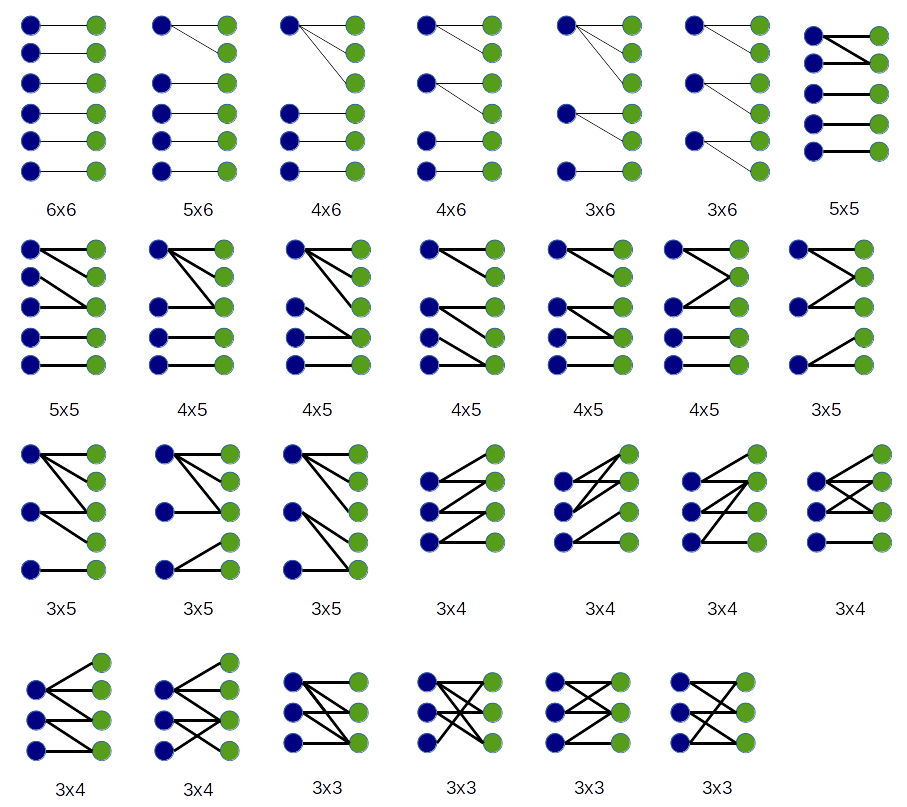
\includegraphics[scale=0.25] {\fig/partial3tree.png}
%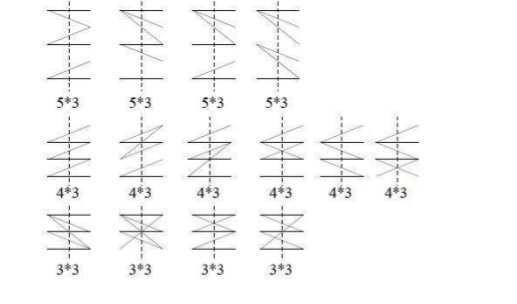
\includegraphics[scale=0.35] {\fig/partial3tree_new_2.png}
\caption{ In each graph above, the vertices of the same color represent points
in the same point-set $A$ (or $B$) in Problem (\cone, \ctwo) and form a complete graph (whose edges are not shown).
Edges between vertices indicate point pairs whose distance is in the preferred
interval, i.e., the constraint is active. For $k=2$, all active constraint
graphs are isomorphic to subgraphs of the ones shown. The graphs above are
rigid and correspond to generically rigid 0-dimensional active constraint
regions. The label $m_1 \times m_2$ below each active constraint graph
indicates that $m_1$ points in the first point-set and $m_2$ points in the
second point-set participate in the active constraints.} 
\label{fig:3-trees}
\end{figure}


The quadratic and linear polynomials defined in Theorem \ref{thm} arise from
simple edge-length (metric) relationships within all triangles and tetrahedra
and are called \emph{tetrahedral inequalities}, and the explicit bounds
mentioned in the theorem are called \emph{tetrahedral bounds}. EASAL leverages
this efficient computation of the convex bounds enhanced by the Theorem 5.1.3
in \cite{ugandhar}, described in Section \ref{sec:tetrahedralbounds}.  It turns
out that, for small $k$, almost all active constraint graphs arising from
Problem (\cone, \ctwo) are partial 3-trees and thus their regions have a convex
Cayley parametrization. Specifically (see \figref{fig:3-trees}), all the active
constraint graphs with 1, 2 and 3 active constraints (5D, 4D and 3D atlas
regions) are partial 3-trees. $86\%$ of active constraint graphs with 4 active
constraints (2D atlas regions) and $70\%$ of active constraint graphs with 5
active constraints (1D atlas regions) are partial 3-trees. Since, regions with 6
active constraints (0D atlas regions) have finite realization spaces, Cayley
parametrization is irrelevant. Section \ref{sec:raytracing} describes how we
find realizations when the active constraint graph is not a partial-3-tree.


Although most active constraint graphs have convex Cayley configuration spaces,
the feasible region is a non-convex subset created by cutting out a region
defined by other constraints of type \cone. Each such constraint is between a
pair of points, one from each point-set, that is neither an active constraint
nor a Cayley parameter in the active constraint graph. However, the regions
that are cut out typically have a (potentially different) convex Cayley
parametrization. This can be seen in \figref{fig:pctreeSpace} where the Cayley
configuration space of the node in the center has a hole cut out because of
constraint violations by point pairs that are neither Cayley parameters nor
edges in the active constraint graph.


\subsubsection{\toytwod\ contd}
Here, the active constraint graph shown in \figref{fig:2DToy} is used to
illustrate Cayley convexification. Since that example is in $\mathbb{R}^2$,
2-trees serve the purpose of 3-trees used in EASAL \cite{SiGa:2010}. A
\emph{complete 2-tree} is any graph obtained by starting with an edge and
successively pasting a triangle onto an edge in the current graph. A
\emph{partial 2-tree} is any subgraph of complete 2-tree.

Consider the partial 2-tree linkage shown in \figref{fig:2DCayley} (left).  To
represent the configuration space of this flexible linkage, we add the
non-edges $e1$ and $e2$, shown with dotted lines, to complete the 2-tree. This
not only makes the linkage rigid, but its realization is easy by a
straightforward ruler and compass construction, solving two quadratics at a
time. The non-edges $e1$ and $e2$ are the Cayley parameters and correspond to
independent flexes.  \figref{fig:2DCayley} (right) shows the convex Cayley configuration
space corresponding to this linkage. 


\begin{figure}[h]
\begin{center}
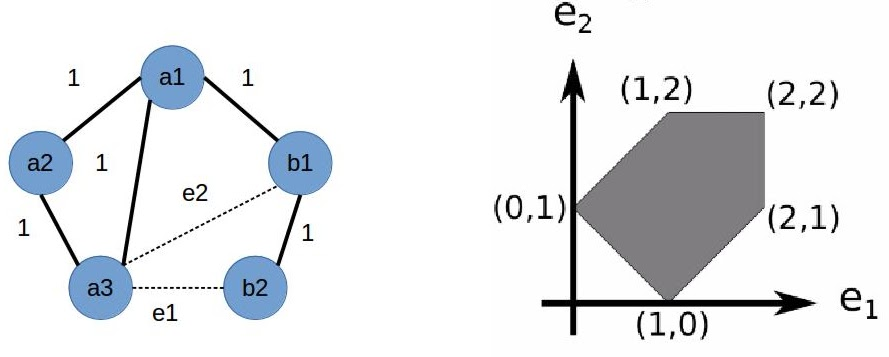
\includegraphics[width=.6\linewidth]{\fig/ConfigSpaceExample.jpg}
\end{center}
\caption{\exref{\toytwod} viewed as
(\IL) a linkage in $\mathbb{R}^2$ (see text for description). (\IR)
The 2D convex Cayley configuration space for the linkage and the chosen Cayley
parameters $e1$ and $e2$. The shaded area delineates the realizable lengths of
$e1$ and $e2$.} 
\label{fig:2DCayley}
\end{figure}


If the edges in the graph in \figref{fig:2DCayley} (left) were assigned length
intervals instead of fixed lengths, yielding an active constraint linkage, the
resulting configuration space would continue to be convex, but would be 7
dimensional. However, when these intervals are relatively small in comparison
to the edge lengths, the Cayley configuration space remains effectively 2
dimensional.


\subsubsection{Realization: Computing Cartesian Configurations from a Cayley Configuration}
\label{sec:realization} 
The addition of the Cayley parameter non-edges to the active constraint graph
yields a complete 3-tree. This reduces computation of the Cartesian
realizations of a Cayley configuration (a tuple of Cayley parameter length
values) to realizing a complete 3-tree linkage. Realizing a complete 3-tree
linkage with $i$ tetrahedra reduces to placing $i$ new points one at a time
using 3 distance constraints between a new point and 3 already placed points.
For each new point we solve the quadratic system for intersecting 3 spheres
resulting in two possible placements of the new point. This yields $2^i$
possible realizations of the Cayley configuration. A \emph{flip} associated
with the Cayley configuration space consists of Cartesian realizations of all
Cayley configurations restricted to one of these $2^i$ placements
\cite{Ozkan2014MainEasal}. 

%XXXXXXXXXXX
%\figref{fig:pctreeSweep} and \figref{fig:boundarySweeps} show the Cayley configuration space as well as the
%Cartesian realization space (flips shown as sweeps) of an atlas region. Ancestor and
%descendant regions are also shown.
